\documentclass[1p]{elsarticle_modified}
%\bibliographystyle{elsarticle-num}

%\usepackage[colorlinks]{hyperref}
%\usepackage{abbrmath_seonhwa} %\Abb, \Ascr, \Acal ,\Abf, \Afrak
\usepackage{amsfonts}
\usepackage{amssymb}
\usepackage{amsmath}
\usepackage{amsthm}
\usepackage{scalefnt}
\usepackage{amsbsy}
\usepackage{kotex}
\usepackage{caption}
\usepackage{subfig}
\usepackage{color}
\usepackage{graphicx}
\usepackage{xcolor} %% white, black, red, green, blue, cyan, magenta, yellow
\usepackage{float}
\usepackage{setspace}
\usepackage{hyperref}

\usepackage{tikz}
\usetikzlibrary{arrows}

\usepackage{multirow}
\usepackage{array} % fixed length table
\usepackage{hhline}

%%%%%%%%%%%%%%%%%%%%%
\makeatletter
\renewcommand*\env@matrix[1][\arraystretch]{%
	\edef\arraystretch{#1}%
	\hskip -\arraycolsep
	\let\@ifnextchar\new@ifnextchar
	\array{*\c@MaxMatrixCols c}}
\makeatother %https://tex.stackexchange.com/questions/14071/how-can-i-increase-the-line-spacing-in-a-matrix
%%%%%%%%%%%%%%%

\usepackage[normalem]{ulem}

\newcommand{\msout}[1]{\ifmmode\text{\sout{\ensuremath{#1}}}\else\sout{#1}\fi}
%SOURCE: \msout is \stkout macro in https://tex.stackexchange.com/questions/20609/strikeout-in-math-mode

\newcommand{\cancel}[1]{
	\ifmmode
	{\color{red}\msout{#1}}
	\else
	{\color{red}\sout{#1}}
	\fi
}

\newcommand{\add}[1]{
	{\color{blue}\uwave{#1}}
}

\newcommand{\replace}[2]{
	\ifmmode
	{\color{red}\msout{#1}}{\color{blue}\uwave{#2}}
	\else
	{\color{red}\sout{#1}}{\color{blue}\uwave{#2}}
	\fi
}

\newcommand{\Sol}{\mathcal{S}} %segment
\newcommand{\D}{D} %diagram
\newcommand{\A}{\mathcal{A}} %arc


%%%%%%%%%%%%%%%%%%%%%%%%%%%%%5 test

\def\sl{\operatorname{\textup{SL}}(2,\Cbb)}
\def\psl{\operatorname{\textup{PSL}}(2,\Cbb)}
\def\quan{\mkern 1mu \triangleright \mkern 1mu}

\theoremstyle{definition}
\newtheorem{thm}{Theorem}[section]
\newtheorem{prop}[thm]{Proposition}
\newtheorem{lem}[thm]{Lemma}
\newtheorem{ques}[thm]{Question}
\newtheorem{cor}[thm]{Corollary}
\newtheorem{defn}[thm]{Definition}
\newtheorem{exam}[thm]{Example}
\newtheorem{rmk}[thm]{Remark}
\newtheorem{alg}[thm]{Algorithm}

\newcommand{\I}{\sqrt{-1}}
\begin{document}

%\begin{frontmatter}
%
%\title{Boundary parabolic representations of knots up to 8 crossings}
%
%%% Group authors per affiliation:
%\author{Yunhi Cho} 
%\address{Department of Mathematics, University of Seoul, Seoul, Korea}
%\ead{yhcho@uos.ac.kr}
%
%
%\author{Seonhwa Kim} %\fnref{s_kim}}
%\address{Center for Geometry and Physics, Institute for Basic Science, Pohang, 37673, Korea}
%\ead{ryeona17@ibs.re.kr}
%
%\author{Hyuk Kim}
%\address{Department of Mathematical Sciences, Seoul National University, Seoul 08826, Korea}
%\ead{hyukkim@snu.ac.kr}
%
%\author{Seokbeom Yoon}
%\address{Department of Mathematical Sciences, Seoul National University, Seoul, 08826,  Korea}
%\ead{sbyoon15@snu.ac.kr}
%
%\begin{abstract}
%We find all boundary parabolic representation of knots up to 8 crossings.
%
%\end{abstract}
%\begin{keyword}
%    \MSC[2010] 57M25 
%\end{keyword}
%
%\end{frontmatter}

%\linenumbers
%\tableofcontents
%
\newcommand\colored[1]{\textcolor{white}{\rule[-0.35ex]{0.8em}{1.4ex}}\kern-0.8em\color{red} #1}%
%\newcommand\colored[1]{\textcolor{white}{ #1}\kern-2.17ex	\textcolor{white}{ #1}\kern-1.81ex	\textcolor{white}{ #1}\kern-2.15ex\color{red}#1	}

{\Large $\underline{11a_{121}~(K11a_{121})}$}

\setlength{\tabcolsep}{10pt}
\renewcommand{\arraystretch}{1.6}
\vspace{1cm}\begin{tabular}{m{100pt}>{\centering\arraybackslash}m{274pt}}
\multirow{5}{120pt}{
	\centering
	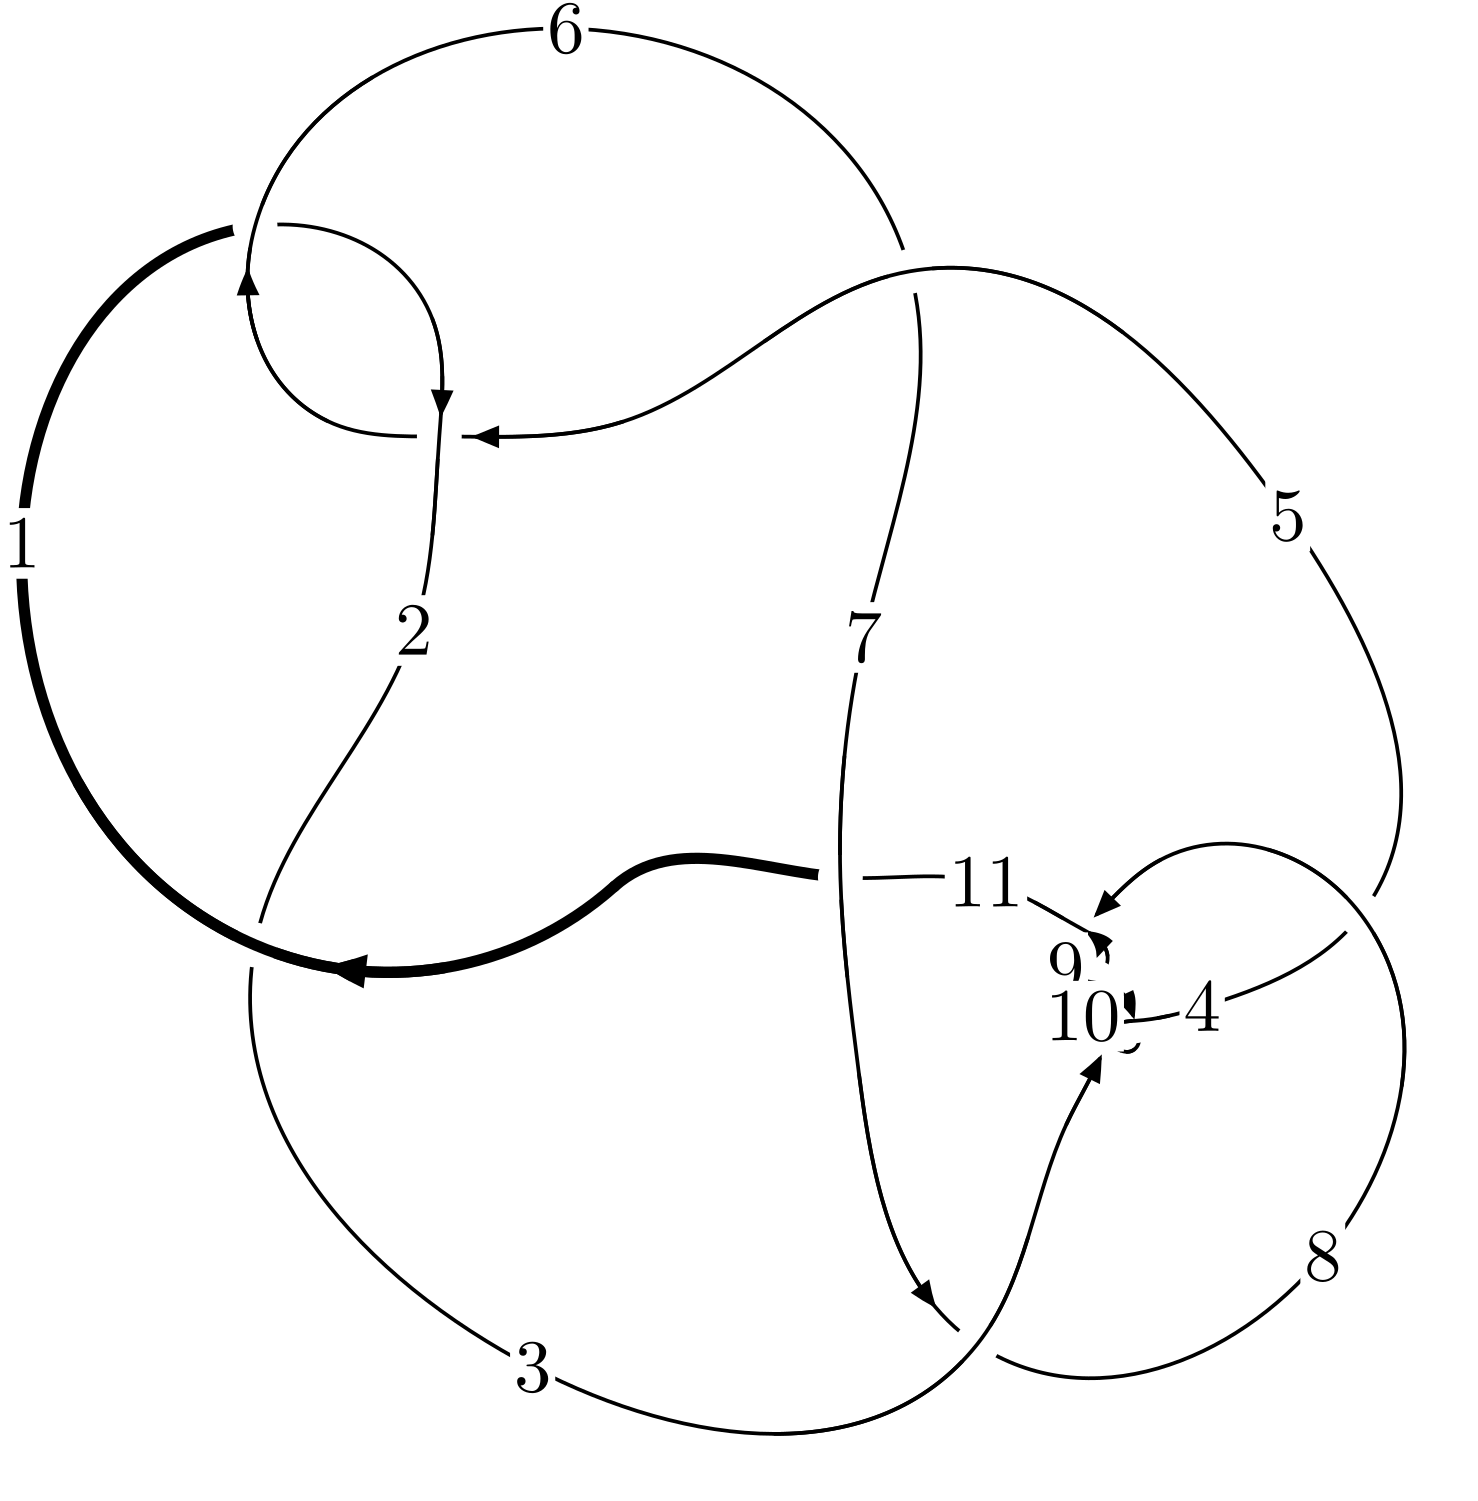
\includegraphics[width=112pt]{../../../GIT/diagram.site/Diagrams/png/370_11a_121.png}\\
\ \ \ A knot diagram\footnotemark}&
\allowdisplaybreaks
\textbf{Linearized knot diagam} \\
\cline{2-2}
 &
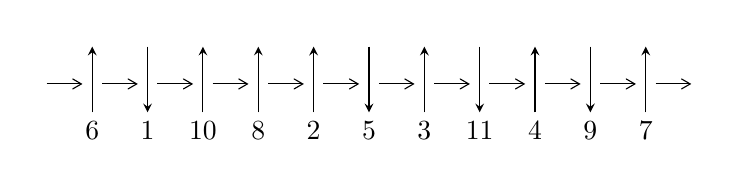
\begin{tikzpicture}[x=20pt, y=17pt]
	% nodes
	\node (C0) at (0, 0) {};
	\node (C1) at (1, 0) {};
	\node (C1U) at (1, +1) {};
	\node (C1D) at (1, -1) {6};

	\node (C2) at (2, 0) {};
	\node (C2U) at (2, +1) {};
	\node (C2D) at (2, -1) {1};

	\node (C3) at (3, 0) {};
	\node (C3U) at (3, +1) {};
	\node (C3D) at (3, -1) {10};

	\node (C4) at (4, 0) {};
	\node (C4U) at (4, +1) {};
	\node (C4D) at (4, -1) {8};

	\node (C5) at (5, 0) {};
	\node (C5U) at (5, +1) {};
	\node (C5D) at (5, -1) {2};

	\node (C6) at (6, 0) {};
	\node (C6U) at (6, +1) {};
	\node (C6D) at (6, -1) {5};

	\node (C7) at (7, 0) {};
	\node (C7U) at (7, +1) {};
	\node (C7D) at (7, -1) {3};

	\node (C8) at (8, 0) {};
	\node (C8U) at (8, +1) {};
	\node (C8D) at (8, -1) {11};

	\node (C9) at (9, 0) {};
	\node (C9U) at (9, +1) {};
	\node (C9D) at (9, -1) {4};

	\node (C10) at (10, 0) {};
	\node (C10U) at (10, +1) {};
	\node (C10D) at (10, -1) {9};

	\node (C11) at (11, 0) {};
	\node (C11U) at (11, +1) {};
	\node (C11D) at (11, -1) {7};
	\node (C12) at (12, 0) {};

	% arrows
	\draw[->,>={angle 60}]
	(C0) edge (C1) (C1) edge (C2) (C2) edge (C3) (C3) edge (C4) (C4) edge (C5) (C5) edge (C6) (C6) edge (C7) (C7) edge (C8) (C8) edge (C9) (C9) edge (C10) (C10) edge (C11) (C11) edge (C12) ;	\draw[->,>=stealth]
	(C1D) edge (C1U) (C2U) edge (C2D) (C3D) edge (C3U) (C4D) edge (C4U) (C5D) edge (C5U) (C6U) edge (C6D) (C7D) edge (C7U) (C8U) edge (C8D) (C9D) edge (C9U) (C10U) edge (C10D) (C11D) edge (C11U) ;
	\end{tikzpicture} \\
\hhline{~~} \\& 
\textbf{Solving Sequence} \\ \cline{2-2} 
 &
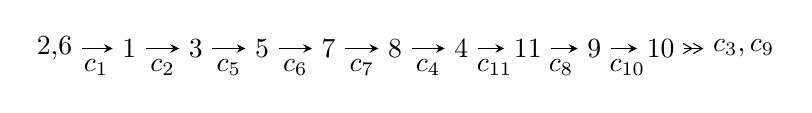
\begin{tikzpicture}[x=24pt, y=7pt]
	% node
	\node (A0) at (-1/8, 0) {2,6};
	\node (A1) at (1, 0) {1};
	\node (A2) at (2, 0) {3};
	\node (A3) at (3, 0) {5};
	\node (A4) at (4, 0) {7};
	\node (A5) at (5, 0) {8};
	\node (A6) at (6, 0) {4};
	\node (A7) at (7, 0) {11};
	\node (A8) at (8, 0) {9};
	\node (A9) at (9, 0) {10};
	\node (C1) at (1/2, -1) {$c_{1}$};
	\node (C2) at (3/2, -1) {$c_{2}$};
	\node (C3) at (5/2, -1) {$c_{5}$};
	\node (C4) at (7/2, -1) {$c_{6}$};
	\node (C5) at (9/2, -1) {$c_{7}$};
	\node (C6) at (11/2, -1) {$c_{4}$};
	\node (C7) at (13/2, -1) {$c_{11}$};
	\node (C8) at (15/2, -1) {$c_{8}$};
	\node (C9) at (17/2, -1) {$c_{10}$};
	\node (A10) at (41/4, 0) {$c_{3},c_{9}$};

	% edge
	\draw[->,>=stealth]	
	(A0) edge (A1) (A1) edge (A2) (A2) edge (A3) (A3) edge (A4) (A4) edge (A5) (A5) edge (A6) (A6) edge (A7) (A7) edge (A8) (A8) edge (A9) ;
	\draw[->>,>={angle 60}]	
	(A9) edge (A10);
\end{tikzpicture} \\ 

\end{tabular} \\

\footnotetext{
The image of knot diagram is generated by the software ``\textbf{Draw programme}" developed by Andrew Bartholomew(\url{http://www.layer8.co.uk/maths/draw/index.htm\#Running-draw}), where we modified some parts for our purpose(\url{https://github.com/CATsTAILs/LinksPainter}).
}\phantom \\ \newline 
\centering \textbf{Ideals for irreducible components\footnotemark of $X_{\text{par}}$} 
 
\begin{align*}
I^u_{1}&=\langle 
u^{11}+2 u^9+4 u^7+4 u^5- u^4+3 u^3- u^2+2 u-1\rangle \\
I^u_{2}&=\langle 
u^{48}- u^{47}+\cdots+2 u+1\rangle \\
\\
\end{align*}
\raggedright * 2 irreducible components of $\dim_{\mathbb{C}}=0$, with total 59 representations.\\
\footnotetext{All coefficients of polynomials are rational numbers. But the coefficients are sometimes approximated in decimal forms when there is not enough margin.}
\newpage
\renewcommand{\arraystretch}{1}
\centering \section*{I. $I^u_{1}= \langle u^{11}+2 u^9+4 u^7+4 u^5- u^4+3 u^3- u^2+2 u-1 \rangle$}
\flushleft \textbf{(i) Arc colorings}\\
\begin{tabular}{m{7pt} m{180pt} m{7pt} m{180pt} }
\flushright $a_{2}=$&$\begin{pmatrix}1\\0\end{pmatrix}$ \\
\flushright $a_{6}=$&$\begin{pmatrix}0\\u\end{pmatrix}$ \\
\flushright $a_{1}=$&$\begin{pmatrix}1\\u^2\end{pmatrix}$ \\
\flushright $a_{3}=$&$\begin{pmatrix}u^2+1\\u^4\end{pmatrix}$ \\
\flushright $a_{5}=$&$\begin{pmatrix}- u\\u\end{pmatrix}$ \\
\flushright $a_{7}=$&$\begin{pmatrix}- u^3\\u^3+u\end{pmatrix}$ \\
\flushright $a_{8}=$&$\begin{pmatrix}u^9+2 u^7+3 u^5+2 u^3+u\\- u^9-2 u^7-3 u^5+u^4-2 u^3+u^2- u+1\end{pmatrix}$ \\
\flushright $a_{4}=$&$\begin{pmatrix}u^8- u^7+u^6-2 u^5+2 u^4-2 u^3+u^2-2 u\\- u^9- u^8- u^7- u^6- u^5-2 u^4- u^2+u\end{pmatrix}$ \\
\flushright $a_{11}=$&$\begin{pmatrix}- u^8- u^6- u^4+1\\u^8+2 u^6+2 u^4+2 u^2\end{pmatrix}$ \\
\flushright $a_{9}=$&$\begin{pmatrix}u^{10}+u^9+u^8+2 u^7+u^6+3 u^5+2 u^3- u^2+u\\- u^{10}- u^9-2 u^8-2 u^7-2 u^6-3 u^5- u^4-2 u^3+u^2- u+1\end{pmatrix}$ \\
\flushright $a_{10}=$&$\begin{pmatrix}u^{10}+2 u^8+u^7+3 u^6+u^5+2 u^4+u^3+u^2+u\\- u^8- u^7- u^6- u^5- u^4- u^3- u+1\end{pmatrix}$\\ \flushright $a_{10}=$&$\begin{pmatrix}u^{10}+2 u^8+u^7+3 u^6+u^5+2 u^4+u^3+u^2+u\\- u^8- u^7- u^6- u^5- u^4- u^3- u+1\end{pmatrix}$\\&\end{tabular}
\flushleft \textbf{(ii) Obstruction class $= -1$}\\~\\
\flushleft \textbf{(iii) Cusp Shapes $= 4 u^{10}+4 u^9+4 u^8+8 u^7+12 u^6+16 u^5+8 u^4+8 u^3+4 u^2+8 u+6$}\\~\\
\newpage\renewcommand{\arraystretch}{1}
\flushleft \textbf{(iv) u-Polynomials at the component}\newline \\
\begin{tabular}{m{50pt}|m{274pt}}
Crossings & \hspace{64pt}u-Polynomials at each crossing \\
\hline $$\begin{aligned}c_{1},c_{3},c_{5}\\c_{9}\end{aligned}$$&$\begin{aligned}
&u^{11}+2 u^9+4 u^7+4 u^5- u^4+3 u^3- u^2+2 u-1
\end{aligned}$\\
\hline $$\begin{aligned}c_{2},c_{6},c_{8}\\c_{10}\end{aligned}$$&$\begin{aligned}
&u^{11}+4 u^{10}+\cdots+2 u-1
\end{aligned}$\\
\hline $$\begin{aligned}c_{4},c_{11}\end{aligned}$$&$\begin{aligned}
&u^{11}+2 u^9-2 u^8+10 u^7+12 u^5-3 u^4+5 u^3- u^2-1
\end{aligned}$\\
\hline $$\begin{aligned}c_{7}\end{aligned}$$&$\begin{aligned}
&u^{11}-7 u^{10}+\cdots+28 u-8
\end{aligned}$\\
\hline
\end{tabular}\\~\\
\newpage\renewcommand{\arraystretch}{1}
\flushleft \textbf{(v) Riley Polynomials at the component}\newline \\
\begin{tabular}{m{50pt}|m{274pt}}
Crossings & \hspace{64pt}Riley Polynomials at each crossing \\
\hline $$\begin{aligned}c_{1},c_{3},c_{5}\\c_{9}\end{aligned}$$&$\begin{aligned}
&y^{11}+4 y^{10}+\cdots+2 y-1
\end{aligned}$\\
\hline $$\begin{aligned}c_{2},c_{6},c_{8}\\c_{10}\end{aligned}$$&$\begin{aligned}
&y^{11}+8 y^{10}+\cdots+22 y-1
\end{aligned}$\\
\hline $$\begin{aligned}c_{4},c_{11}\end{aligned}$$&$\begin{aligned}
&y^{11}+4 y^{10}+\cdots-2 y-1
\end{aligned}$\\
\hline $$\begin{aligned}c_{7}\end{aligned}$$&$\begin{aligned}
&y^{11}-3 y^{10}+\cdots+48 y-64
\end{aligned}$\\
\hline
\end{tabular}\\~\\
\newpage\flushleft \textbf{(vi) Complex Volumes and Cusp Shapes}
$$\begin{array}{c|c|c}  
\text{Solutions to }I^u_{1}& \I (\text{vol} + \sqrt{-1}CS) & \text{Cusp shape}\\
 \hline 
\begin{aligned}
u &= -0.111009 + 1.030810 I\end{aligned}
 & -5.93919 - 3.55367 I & -6.35449 + 4.86751 I \\ \hline\begin{aligned}
u &= -0.111009 - 1.030810 I\end{aligned}
 & -5.93919 + 3.55367 I & -6.35449 - 4.86751 I \\ \hline\begin{aligned}
u &= \phantom{-}0.594105 + 0.723647 I\end{aligned}
 & \phantom{-}1.48764 + 1.96750 I & \phantom{-}4.49213 - 3.23948 I \\ \hline\begin{aligned}
u &= \phantom{-}0.594105 - 0.723647 I\end{aligned}
 & \phantom{-}1.48764 - 1.96750 I & \phantom{-}4.49213 + 3.23948 I \\ \hline\begin{aligned}
u &= -0.817015 + 0.707633 I\end{aligned}
 & \phantom{-}6.68078 + 3.13136 I & \phantom{-}8.76083 - 0.56604 I \\ \hline\begin{aligned}
u &= -0.817015 - 0.707633 I\end{aligned}
 & \phantom{-}6.68078 - 3.13136 I & \phantom{-}8.76083 + 0.56604 I \\ \hline\begin{aligned}
u &= -0.617277 + 0.966546 I\end{aligned}
 & -0.07920 - 7.68222 I & \phantom{-}0.97285 + 8.49443 I \\ \hline\begin{aligned}
u &= -0.617277 - 0.966546 I\end{aligned}
 & -0.07920 + 7.68222 I & \phantom{-}0.97285 - 8.49443 I \\ \hline\begin{aligned}
u &= \phantom{-}0.729012 + 1.011350 I\end{aligned}
 & \phantom{-}4.8176 + 14.7555 I & \phantom{-}5.24582 - 10.31160 I \\ \hline\begin{aligned}
u &= \phantom{-}0.729012 - 1.011350 I\end{aligned}
 & \phantom{-}4.8176 - 14.7555 I & \phantom{-}5.24582 + 10.31160 I \\ \hline\begin{aligned}
u &= \phantom{-}0.444369\phantom{ +0.000000I}\end{aligned}
 & \phantom{-}0.869046\phantom{ +0.000000I} & \phantom{-}11.7660\phantom{ +0.000000I}\\
 \hline 
 \end{array}$$\newpage\newpage\renewcommand{\arraystretch}{1}
\centering \section*{II. $I^u_{2}= \langle u^{48}- u^{47}+\cdots+2 u+1 \rangle$}
\flushleft \textbf{(i) Arc colorings}\\
\begin{tabular}{m{7pt} m{180pt} m{7pt} m{180pt} }
\flushright $a_{2}=$&$\begin{pmatrix}1\\0\end{pmatrix}$ \\
\flushright $a_{6}=$&$\begin{pmatrix}0\\u\end{pmatrix}$ \\
\flushright $a_{1}=$&$\begin{pmatrix}1\\u^2\end{pmatrix}$ \\
\flushright $a_{3}=$&$\begin{pmatrix}u^2+1\\u^4\end{pmatrix}$ \\
\flushright $a_{5}=$&$\begin{pmatrix}- u\\u\end{pmatrix}$ \\
\flushright $a_{7}=$&$\begin{pmatrix}- u^3\\u^3+u\end{pmatrix}$ \\
\flushright $a_{8}=$&$\begin{pmatrix}u^9+2 u^7+3 u^5+2 u^3+u\\u^{11}+u^9+2 u^7+u^5+u^3+u\end{pmatrix}$ \\
\flushright $a_{4}=$&$\begin{pmatrix}- u^{21}-4 u^{19}+\cdots-2 u^3- u\\- u^{23}-3 u^{21}+\cdots-2 u^3+u\end{pmatrix}$ \\
\flushright $a_{11}=$&$\begin{pmatrix}- u^8- u^6- u^4+1\\u^8+2 u^6+2 u^4+2 u^2\end{pmatrix}$ \\
\flushright $a_{9}=$&$\begin{pmatrix}- u^{27}-4 u^{25}+\cdots+10 u^5+3 u^3\\u^{27}+5 u^{25}+\cdots- u^3+u\end{pmatrix}$ \\
\flushright $a_{10}=$&$\begin{pmatrix}- u^{46}-7 u^{44}+\cdots-4 u^4+1\\u^{46}+8 u^{44}+\cdots+4 u^4+u^2\end{pmatrix}$\\ \flushright $a_{10}=$&$\begin{pmatrix}- u^{46}-7 u^{44}+\cdots-4 u^4+1\\u^{46}+8 u^{44}+\cdots+4 u^4+u^2\end{pmatrix}$\\&\end{tabular}
\flushleft \textbf{(ii) Obstruction class $= -1$}\\~\\
\flushleft \textbf{(iii) Cusp Shapes $= 4 u^{45}+28 u^{43}+132 u^{41}+448 u^{39}+1224 u^{37}+2772 u^{35}+5348 u^{33}+8916 u^{31}+12948 u^{29}-4 u^{28}+16456 u^{27}-20 u^{26}+18292 u^{25}-68 u^{24}+17704 u^{23}-164 u^{22}+14776 u^{21}-308 u^{20}+10428 u^{19}-468 u^{18}+6020 u^{17}-576 u^{16}+2644 u^{15}-580 u^{14}+720 u^{13}-468 u^{12}-288 u^{10}-88 u^9-124 u^8-4 u^7-24 u^6+36 u^5+8 u^4+24 u^3+4 u^2+4 u+2$}\\~\\
\newpage\renewcommand{\arraystretch}{1}
\flushleft \textbf{(iv) u-Polynomials at the component}\newline \\
\begin{tabular}{m{50pt}|m{274pt}}
Crossings & \hspace{64pt}u-Polynomials at each crossing \\
\hline $$\begin{aligned}c_{1},c_{3},c_{5}\\c_{9}\end{aligned}$$&$\begin{aligned}
&u^{48}- u^{47}+\cdots+2 u+1
\end{aligned}$\\
\hline $$\begin{aligned}c_{2},c_{6},c_{8}\\c_{10}\end{aligned}$$&$\begin{aligned}
&u^{48}+15 u^{47}+\cdots+8 u^3+1
\end{aligned}$\\
\hline $$\begin{aligned}c_{4},c_{11}\end{aligned}$$&$\begin{aligned}
&u^{48}+5 u^{47}+\cdots+12 u+1
\end{aligned}$\\
\hline $$\begin{aligned}c_{7}\end{aligned}$$&$\begin{aligned}
&(u^{24}+3 u^{23}+\cdots+18 u+7)^{2}
\end{aligned}$\\
\hline
\end{tabular}\\~\\
\newpage\renewcommand{\arraystretch}{1}
\flushleft \textbf{(v) Riley Polynomials at the component}\newline \\
\begin{tabular}{m{50pt}|m{274pt}}
Crossings & \hspace{64pt}Riley Polynomials at each crossing \\
\hline $$\begin{aligned}c_{1},c_{3},c_{5}\\c_{9}\end{aligned}$$&$\begin{aligned}
&y^{48}+15 y^{47}+\cdots+8 y^3+1
\end{aligned}$\\
\hline $$\begin{aligned}c_{2},c_{6},c_{8}\\c_{10}\end{aligned}$$&$\begin{aligned}
&y^{48}+35 y^{47}+\cdots+88 y^2+1
\end{aligned}$\\
\hline $$\begin{aligned}c_{4},c_{11}\end{aligned}$$&$\begin{aligned}
&y^{48}-5 y^{47}+\cdots-24 y+1
\end{aligned}$\\
\hline $$\begin{aligned}c_{7}\end{aligned}$$&$\begin{aligned}
&(y^{24}-9 y^{23}+\cdots-212 y+49)^{2}
\end{aligned}$\\
\hline
\end{tabular}\\~\\
\newpage\flushleft \textbf{(vi) Complex Volumes and Cusp Shapes}
$$\begin{array}{c|c|c}  
\text{Solutions to }I^u_{2}& \I (\text{vol} + \sqrt{-1}CS) & \text{Cusp shape}\\
 \hline 
\begin{aligned}
u &= -0.447030 + 0.894068 I\end{aligned}
 & \phantom{-}0.85406 + 3.28062 I & \phantom{-}1.88284 - 1.76353 I \\ \hline\begin{aligned}
u &= -0.447030 - 0.894068 I\end{aligned}
 & \phantom{-}0.85406 - 3.28062 I & \phantom{-}1.88284 + 1.76353 I \\ \hline\begin{aligned}
u &= -0.037970 + 1.018320 I\end{aligned}
 & -3.47428 + 2.08425 I & -3.81787 - 2.59078 I \\ \hline\begin{aligned}
u &= -0.037970 - 1.018320 I\end{aligned}
 & -3.47428 - 2.08425 I & -3.81787 + 2.59078 I \\ \hline\begin{aligned}
u &= \phantom{-}0.103335 + 0.964930 I\end{aligned}
 & -2.07060 + 1.71275 I & \phantom{-}0.95839 - 4.38827 I \\ \hline\begin{aligned}
u &= \phantom{-}0.103335 - 0.964930 I\end{aligned}
 & -2.07060 - 1.71275 I & \phantom{-}0.95839 + 4.38827 I \\ \hline\begin{aligned}
u &= \phantom{-}0.709249 + 0.753994 I\end{aligned}
 & \phantom{-}1.54659 + 2.07802 I & \phantom{-}3.74247 - 4.14356 I \\ \hline\begin{aligned}
u &= \phantom{-}0.709249 - 0.753994 I\end{aligned}
 & \phantom{-}1.54659 - 2.07802 I & \phantom{-}3.74247 + 4.14356 I \\ \hline\begin{aligned}
u &= \phantom{-}0.161802 + 1.028080 I\end{aligned}
 & \phantom{-}0.15229 + 3.45771 I & \phantom{-}1.61918 - 3.33537 I \\ \hline\begin{aligned}
u &= \phantom{-}0.161802 - 1.028080 I\end{aligned}
 & \phantom{-}0.15229 - 3.45771 I & \phantom{-}1.61918 + 3.33537 I \\ \hline\begin{aligned}
u &= \phantom{-}0.786969 + 0.691947 I\end{aligned}
 & \phantom{-}0.15229 - 3.45771 I & \phantom{-}1.61918 + 3.33537 I \\ \hline\begin{aligned}
u &= \phantom{-}0.786969 - 0.691947 I\end{aligned}
 & \phantom{-}0.15229 + 3.45771 I & \phantom{-}1.61918 - 3.33537 I \\ \hline\begin{aligned}
u &= -0.156596 + 1.043700 I\end{aligned}
 & -0.78809 - 9.12338 I & -0.18249 + 8.13527 I \\ \hline\begin{aligned}
u &= -0.156596 - 1.043700 I\end{aligned}
 & -0.78809 + 9.12338 I & -0.18249 - 8.13527 I \\ \hline\begin{aligned}
u &= -0.779513 + 0.728650 I\end{aligned}
 & \phantom{-}3.78730 + 1.05884 I & \phantom{-}9.33375 - 1.03697 I \\ \hline\begin{aligned}
u &= -0.779513 - 0.728650 I\end{aligned}
 & \phantom{-}3.78730 - 1.05884 I & \phantom{-}9.33375 + 1.03697 I \\ \hline\begin{aligned}
u &= \phantom{-}0.820160 + 0.698926 I\end{aligned}
 & \phantom{-}5.77023 - 8.94227 I & \phantom{-}7.03302 + 5.48937 I \\ \hline\begin{aligned}
u &= \phantom{-}0.820160 - 0.698926 I\end{aligned}
 & \phantom{-}5.77023 + 8.94227 I & \phantom{-}7.03302 - 5.48937 I \\ \hline\begin{aligned}
u &= -0.559504 + 0.928720 I\end{aligned}
 & -3.47428 - 2.08425 I & -3.81787 + 2.59078 I \\ \hline\begin{aligned}
u &= -0.559504 - 0.928720 I\end{aligned}
 & -3.47428 + 2.08425 I & -3.81787 - 2.59078 I \\ \hline\begin{aligned}
u &= \phantom{-}0.357761 + 0.828361 I\end{aligned}
 & \phantom{-}1.54659 + 2.07802 I & \phantom{-}3.74247 - 4.14356 I \\ \hline\begin{aligned}
u &= \phantom{-}0.357761 - 0.828361 I\end{aligned}
 & \phantom{-}1.54659 - 2.07802 I & \phantom{-}3.74247 + 4.14356 I \\ \hline\begin{aligned}
u &= -0.798379 + 0.782289 I\end{aligned}
 & \phantom{-}7.98533\phantom{ +0.000000I} & \phantom{-}10.04300 + 0. I\phantom{ +0.000000I} \\ \hline\begin{aligned}
u &= -0.798379 - 0.782289 I\end{aligned}
 & \phantom{-}7.98533\phantom{ +0.000000I} & \phantom{-}10.04300 + 0. I\phantom{ +0.000000I} \\ \hline\begin{aligned}
u &= \phantom{-}0.795531 + 0.794799 I\end{aligned}
 & \phantom{-}7.45278 + 5.81585 I & \phantom{-}8.97012 - 5.48927 I \\ \hline\begin{aligned}
u &= \phantom{-}0.795531 - 0.794799 I\end{aligned}
 & \phantom{-}7.45278 - 5.81585 I & \phantom{-}8.97012 + 5.48927 I \\ \hline\begin{aligned}
u &= \phantom{-}0.644764 + 0.924836 I\end{aligned}
 & \phantom{-}0.94545 + 3.01303 I & \phantom{-}3.90717 - 2.47987 I \\ \hline\begin{aligned}
u &= \phantom{-}0.644764 - 0.924836 I\end{aligned}
 & \phantom{-}0.94545 - 3.01303 I & \phantom{-}3.90717 + 2.47987 I \\ \hline\begin{aligned}
u &= \phantom{-}0.684868 + 0.970999 I\end{aligned}
 & \phantom{-}0.85406 + 3.28062 I & \phantom{-}1.88284 - 1.76353 I \\ \hline\begin{aligned}
u &= \phantom{-}0.684868 - 0.970999 I\end{aligned}
 & \phantom{-}0.85406 - 3.28062 I & \phantom{-}1.88284 + 1.76353 I\\
 \hline 
 \end{array}$$\newpage$$\begin{array}{c|c|c}  
\text{Solutions to }I^u_{2}& \I (\text{vol} + \sqrt{-1}CS) & \text{Cusp shape}\\
 \hline 
\begin{aligned}
u &= \phantom{-}0.750786 + 0.945298 I\end{aligned}
 & \phantom{-}6.98909\phantom{ +0.000000I} & \phantom{-}8.15485 + 0. I\phantom{ +0.000000I} \\ \hline\begin{aligned}
u &= \phantom{-}0.750786 - 0.945298 I\end{aligned}
 & \phantom{-}6.98909\phantom{ +0.000000I} & \phantom{-}8.15485 + 0. I\phantom{ +0.000000I} \\ \hline\begin{aligned}
u &= -0.748039 + 0.955471 I\end{aligned}
 & \phantom{-}7.45278 - 5.81585 I & \phantom{-}8.97012 + 5.48927 I \\ \hline\begin{aligned}
u &= -0.748039 - 0.955471 I\end{aligned}
 & \phantom{-}7.45278 + 5.81585 I & \phantom{-}8.97012 - 5.48927 I \\ \hline\begin{aligned}
u &= -0.718495 + 0.983429 I\end{aligned}
 & \phantom{-}3.01107 - 6.72706 I & \phantom{-}7.45449 + 6.34172 I \\ \hline\begin{aligned}
u &= -0.718495 - 0.983429 I\end{aligned}
 & \phantom{-}3.01107 + 6.72706 I & \phantom{-}7.45449 - 6.34172 I \\ \hline\begin{aligned}
u &= \phantom{-}0.712082 + 1.003140 I\end{aligned}
 & -0.78809 + 9.12338 I & \phantom{-0.000000 } 0. - 8.13527 I \\ \hline\begin{aligned}
u &= \phantom{-}0.712082 - 1.003140 I\end{aligned}
 & -0.78809 - 9.12338 I & \phantom{-0.000000 -}0. + 8.13527 I \\ \hline\begin{aligned}
u &= -0.730704 + 1.006040 I\end{aligned}
 & \phantom{-}5.77023 - 8.94227 I & \phantom{-}7.03302 + 5.48937 I \\ \hline\begin{aligned}
u &= -0.730704 - 1.006040 I\end{aligned}
 & \phantom{-}5.77023 + 8.94227 I & \phantom{-}7.03302 - 5.48937 I \\ \hline\begin{aligned}
u &= -0.520871 + 0.529700 I\end{aligned}
 & \phantom{-}0.94545 + 3.01303 I & \phantom{-}3.90717 - 2.47987 I \\ \hline\begin{aligned}
u &= -0.520871 - 0.529700 I\end{aligned}
 & \phantom{-}0.94545 - 3.01303 I & \phantom{-}3.90717 + 2.47987 I \\ \hline\begin{aligned}
u &= -0.619099 + 0.144052 I\end{aligned}
 & \phantom{-}3.01107 - 6.72706 I & \phantom{-}7.45449 + 6.34172 I \\ \hline\begin{aligned}
u &= -0.619099 - 0.144052 I\end{aligned}
 & \phantom{-}3.01107 + 6.72706 I & \phantom{-}7.45449 - 6.34172 I \\ \hline\begin{aligned}
u &= \phantom{-}0.605322 + 0.114770 I\end{aligned}
 & \phantom{-}3.78730 + 1.05884 I & \phantom{-}9.33375 - 1.03697 I \\ \hline\begin{aligned}
u &= \phantom{-}0.605322 - 0.114770 I\end{aligned}
 & \phantom{-}3.78730 - 1.05884 I & \phantom{-}9.33375 + 1.03697 I \\ \hline\begin{aligned}
u &= -0.516429 + 0.228211 I\end{aligned}
 & -2.07060 - 1.71275 I & \phantom{-}0.95839 + 4.38827 I \\ \hline\begin{aligned}
u &= -0.516429 - 0.228211 I\end{aligned}
 & -2.07060 + 1.71275 I & \phantom{-}0.95839 - 4.38827 I\\
 \hline 
 \end{array}$$\newpage
\newpage\renewcommand{\arraystretch}{1}
\centering \section*{ III. u-Polynomials}
\begin{tabular}{m{50pt}|m{274pt}}
Crossings & \hspace{64pt}u-Polynomials at each crossing \\
\hline $$\begin{aligned}c_{1},c_{3},c_{5}\\c_{9}\end{aligned}$$&$\begin{aligned}
&(u^{11}+2 u^9+\cdots+2 u-1)(u^{48}- u^{47}+\cdots+2 u+1)
\end{aligned}$\\
\hline $$\begin{aligned}c_{2},c_{6},c_{8}\\c_{10}\end{aligned}$$&$\begin{aligned}
&(u^{11}+4 u^{10}+\cdots+2 u-1)(u^{48}+15 u^{47}+\cdots+8 u^3+1)
\end{aligned}$\\
\hline $$\begin{aligned}c_{4},c_{11}\end{aligned}$$&$\begin{aligned}
&(u^{11}+2 u^9-2 u^8+10 u^7+12 u^5-3 u^4+5 u^3- u^2-1)\\
&\cdot(u^{48}+5 u^{47}+\cdots+12 u+1)
\end{aligned}$\\
\hline $$\begin{aligned}c_{7}\end{aligned}$$&$\begin{aligned}
&(u^{11}-7 u^{10}+\cdots+28 u-8)(u^{24}+3 u^{23}+\cdots+18 u+7)^{2}
\end{aligned}$\\
\hline
\end{tabular}\newpage\renewcommand{\arraystretch}{1}
\centering \section*{ IV. Riley Polynomials}
\begin{tabular}{m{50pt}|m{274pt}}
Crossings & \hspace{64pt}Riley Polynomials at each crossing \\
\hline $$\begin{aligned}c_{1},c_{3},c_{5}\\c_{9}\end{aligned}$$&$\begin{aligned}
&(y^{11}+4 y^{10}+\cdots+2 y-1)(y^{48}+15 y^{47}+\cdots+8 y^3+1)
\end{aligned}$\\
\hline $$\begin{aligned}c_{2},c_{6},c_{8}\\c_{10}\end{aligned}$$&$\begin{aligned}
&(y^{11}+8 y^{10}+\cdots+22 y-1)(y^{48}+35 y^{47}+\cdots+88 y^2+1)
\end{aligned}$\\
\hline $$\begin{aligned}c_{4},c_{11}\end{aligned}$$&$\begin{aligned}
&(y^{11}+4 y^{10}+\cdots-2 y-1)(y^{48}-5 y^{47}+\cdots-24 y+1)
\end{aligned}$\\
\hline $$\begin{aligned}c_{7}\end{aligned}$$&$\begin{aligned}
&(y^{11}-3 y^{10}+\cdots+48 y-64)(y^{24}-9 y^{23}+\cdots-212 y+49)^{2}
\end{aligned}$\\
\hline
\end{tabular}
\vskip 2pc
\end{document}